\section{Inverse kinematics}

\subsection{Theory}
\label{theory}

For the mathematics explained in this section, it is assumed that both the x-, and the y-axes are horizontal, where the z-axis are vertical. All axes er perpendicular on each other.

When using inverse kinematics, we need to calculate the rotation of the different joints based on a set of coordinates, where the tip of the robotic arm is supposed to be place at the end of its movement. \newline
The first joint of the robotic arm rotates by the base of the robotic arm, which means, that it is only able to manipulate the robotic arms x- and y-axes. Since this is the first joint, there is no other joint that can manipulate the result of this joint. Furthermore, there is no other on the robotic arm, which can manipulate only these axes. All other joints will all manipulate the z-axis, and 1 or 2 of the other axes, depending on the orientation of the first joint.

Because of these things, the angle of the first joint is fairly simple to calculate. Since the tangent of an angle in a unit circle is defined by the Y-coordinate divided by the X- coordinate, the reverse is used to calculate the angle of the first joint:

\begin{equation*}
 \tan(\theta_1) = \frac{\sin(\theta_1)}{\cos(\theta_1)} = \frac{y}{x}
 <=>
 \theta_1 = \tan^{-1}\Big(\frac{y}{x}\Big)   
\end{equation*}

From there, however,  all joint angles needs to be calculated from the outer joints to the inner joints. To do this, we need to take a few steps before we can calculate the actual angles of the remaining 2 joints. First we need to calculate the squared length from the origin to the point the robotic arm must reach. In the Python file it is calculated like this:

\begin{equation*}
    r^2 = \big(x - a_1 \cdot \cos(\theta_1)\big)^2 + \big(y - a_1 \cdot \sin(\theta_1)\big)^2
\end{equation*}

This is done, so it is possible to add a horizontal offset on the link between the 1st and 2nd joint of the robot. This is, however, not the case with this version of the Crustcrawler, which means that the equation will be calculated like this:

\begin{equation*}
    r^2 = x^2 + y^2
\end{equation*}

We're also going to use a calculation, which we're going to call $s$ for now. This is calculated as follows:

\begin{equation*}
    s = z - d_1
\end{equation*}

Which shows that $s$ is basically a new coordinate for z, where joint 2 now has the origin point for the new axis. This means, that $s$ can also be negative.\newline
Now we can also calculate the next step of the inverse kinematics, which looks like the following:

\begin{equation*}
    D = \frac{r^2 + s^2 - a_2^2 - d_4^2}{2 \cdot a_2 \cdot d_4} = \cos(\theta_3)
\end{equation*}

As can be seen, D is also equivalent to to $cos(\theta_3)$. The numerator can also be written as: $r^2 + s^2 - (a_2^2 + d_4^2)$. Since $a_2$ and $d_4$ are the length of the limps, and the rest of the numerator is the length from the 2nd joint to the tip, D will always follow the rule that $-1 \leq D \leq 0$. This is one of the reasons it is not possible to calculate a position of reach for the robot arm, since D is also used in the next calculation:

\begin{equation*}
\sin(\theta_3) = \pm \sqrt{1-D^2}    
\end{equation*}

Therefore, we can see, that if $D < -1$ or possibly $1 < D$, then $\sin(\theta_3)$ would be a complex number, which we cannot use in this instance. Since we now have both $\cos(\theta_3)$ and $\sin(\theta_3)$, we can now calculate $\theta_3$ as shown in the tangent equations further up in this document. Therefore:

\begin{equation*}
    \theta_3 = \tan^{-1}\Bigg(\frac{\pm\sqrt{}1-D^2}{D}\Bigg)
\end{equation*}

Since the $\pm$ shows that this joint can point both upwards and downwards, we're going to make it into only 1 of the 2. This angle decides if the robot is configured to use the elbow up or the elbow down approach, with a negative angle the elbow will point upwards and with positive angle the elbow will point downwards. Since the elbow up approach suits us better the equation ultimately looks like below:

\begin{equation*}
    \theta_3 = \tan^{-1}\Bigg(\frac{-\sqrt{}1-D^2}{D}\Bigg)
\end{equation*}

Now we're left with only 1 calculation, which is to calculate the angle of the 2nd joint, $\theta_2$. This is calculated like shown below:

\begin{equation*}
    \theta_2 = \tan^{-1}\Big(\frac{s}{\sqrt{r^2}}\Big) - \tan^{-1}\bigg(\frac{d_4 \cdot \sin(\theta_3}{a_2 + d_4 \cdot \cos(\theta_3)}\bigg)
\end{equation*}

The first term of the equation is calculated, as if the tip is on just 1 link. This alone would therefore be the calculation, if there was not a joint past joint 2, since it uses it's horizontal and a vertical position. Since there is a 3rd joint past the 2nd joint, we need to compensate for this joint, which is why we have the 2nd term in this equation.\newline
With these equations, we can calculate the different joints of the robot, when it needs to be placed on a certain point in space.

\begin{figure}[h!]
    \centering
    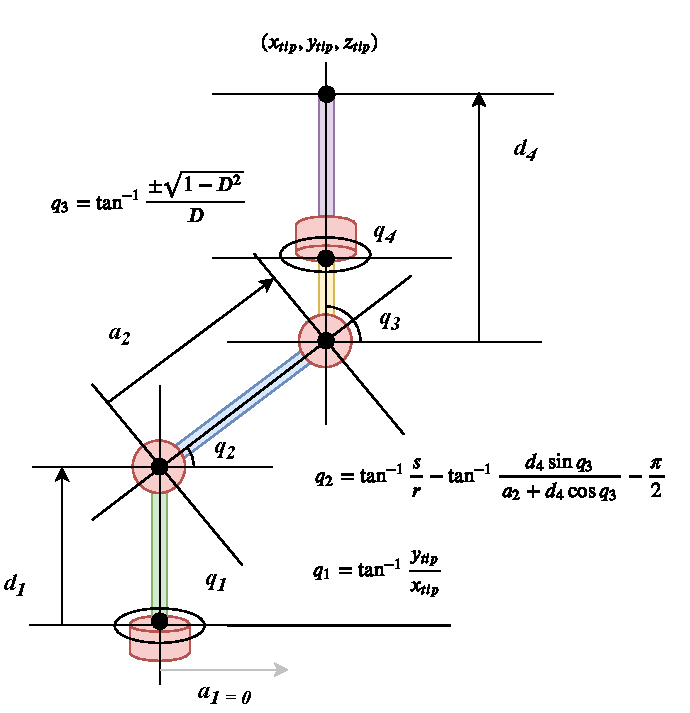
\includegraphics[width=0.8\textwidth]{figures/rob1_inv_kin.pdf}
    \caption{Crustcrawler robot kinematic structure}
    \label{fig:my_label}
\end{figure}

\subsection{ROS implementation}
The function that was used on the robot to make it move via inverse kinematics is listed in this section. The block of code below is a setup with the measured lengths and heights of the robot arm. Some of the numbers have been slightly rounded to make the coordinates easier to interpret. Afterwards the parameter coordinate up into each of the three axes.

The next block of code is the math part of the implementation. Here all the formulas explained in section \ref{theory} are used to calculate the angles of all joints on the robot that are necessary to make the arm edge located on the specific coordinate. What's worth noticing is that the 2nd joint (q2) will subtract pi/2 after its calculations. This is simply to lean the arm and make it face the correct way so the z-axis will be the vertical direction.

\begin{pyminted}
def invkin(xyz):
	d1 = 13.0; # cm (height of 2nd joint)
	a1 = 0.0; # (distance along "y-axis" to 2nd joint)
	a2 = 17.0; # (distance between 2nd and 3rd joints)
	d4 = 20; # (distance from 3rd joint to gripper center - all inclusive, ie. also 4th joint)

	xc = xyz[0]
	yc = xyz[1]
	zc = xyz[2]

	q1 = atan2(yc, xc)

	r2 = (xc - a1*cos(q1))**2 + (yc - a1*\sin(q1))**2
	s = (zc - d1)
	D = (r2 + s**2 - a2**2 - d4**2)/(2*a2*d4)

	q3 = atan2(-sqrt(1-D**2), D) + 0
	q2 = atan2(s, sqrt(r2)) - atan2(d4*sin(q3), a2 + d4*\cos(q3)) - pi/2

	q4 = 0

	return q1,q2,q3,q4
\end{pyminted}

\begin{pyminted}
# initial duration
dur = rospy.Duration(2)

# construct a list of joint positions by calling invkin for each xyz point
for p in xyz_positions:
	jtp = JointTrajectoryPoint(positions=invkin(p), velocities=[0.5]*self.N_JOINTS, time_from_start=dur)
	dur += rospy.Duration(1)
	self.joint_positions.append(jtp)

self.jt = JointTrajectory(joint_names=self.names, points=self.joint_positions)
self.goal = FollowJointTrajectoryGoal( trajectory=self.jt, goal_time_tolerance=dur+rospy.Duration(2) )
\end{pyminted}

\subsection{Test results}

After we succeeded in making the robot move towards the specified coordinates, we were able to test its limits. The robot has a limit on its 3rd joint (q3), where it cannot be angled more than 90 degrees in both directions due to the hardware. Therefore it can only move in an arch, which makes some coordinates impossible to reach. We used the Matlab script to simulate the robot moving from one coordinate to another. With this it was easy to see if the real arm would move inside any unreachable areas. The first example was to move from [0, 25, 20] to [0, 25, 40], which means the x-, y- and z-coordinates respectively. The result can be seen on figure \ref{fig:simulated_arm}.

\begin{figure}[H]
    \centering
    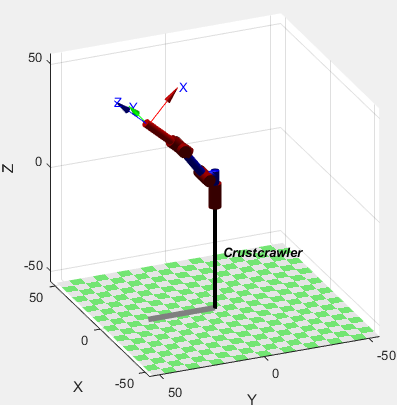
\includegraphics[width=0.6\textwidth]{figures/SimulatedArm.PNG}
    \caption{Crustcrawler simulated in Matlab}
    \label{fig:simulated_arm}
\end{figure}

Figure \ref{fig:matlab} shows the same transition on the real robot as in the simulation. The end result is identical, and the robot can be seen to have the correct x-, y- and z-coordinates.

\begin{figure}[H]
    \centering
    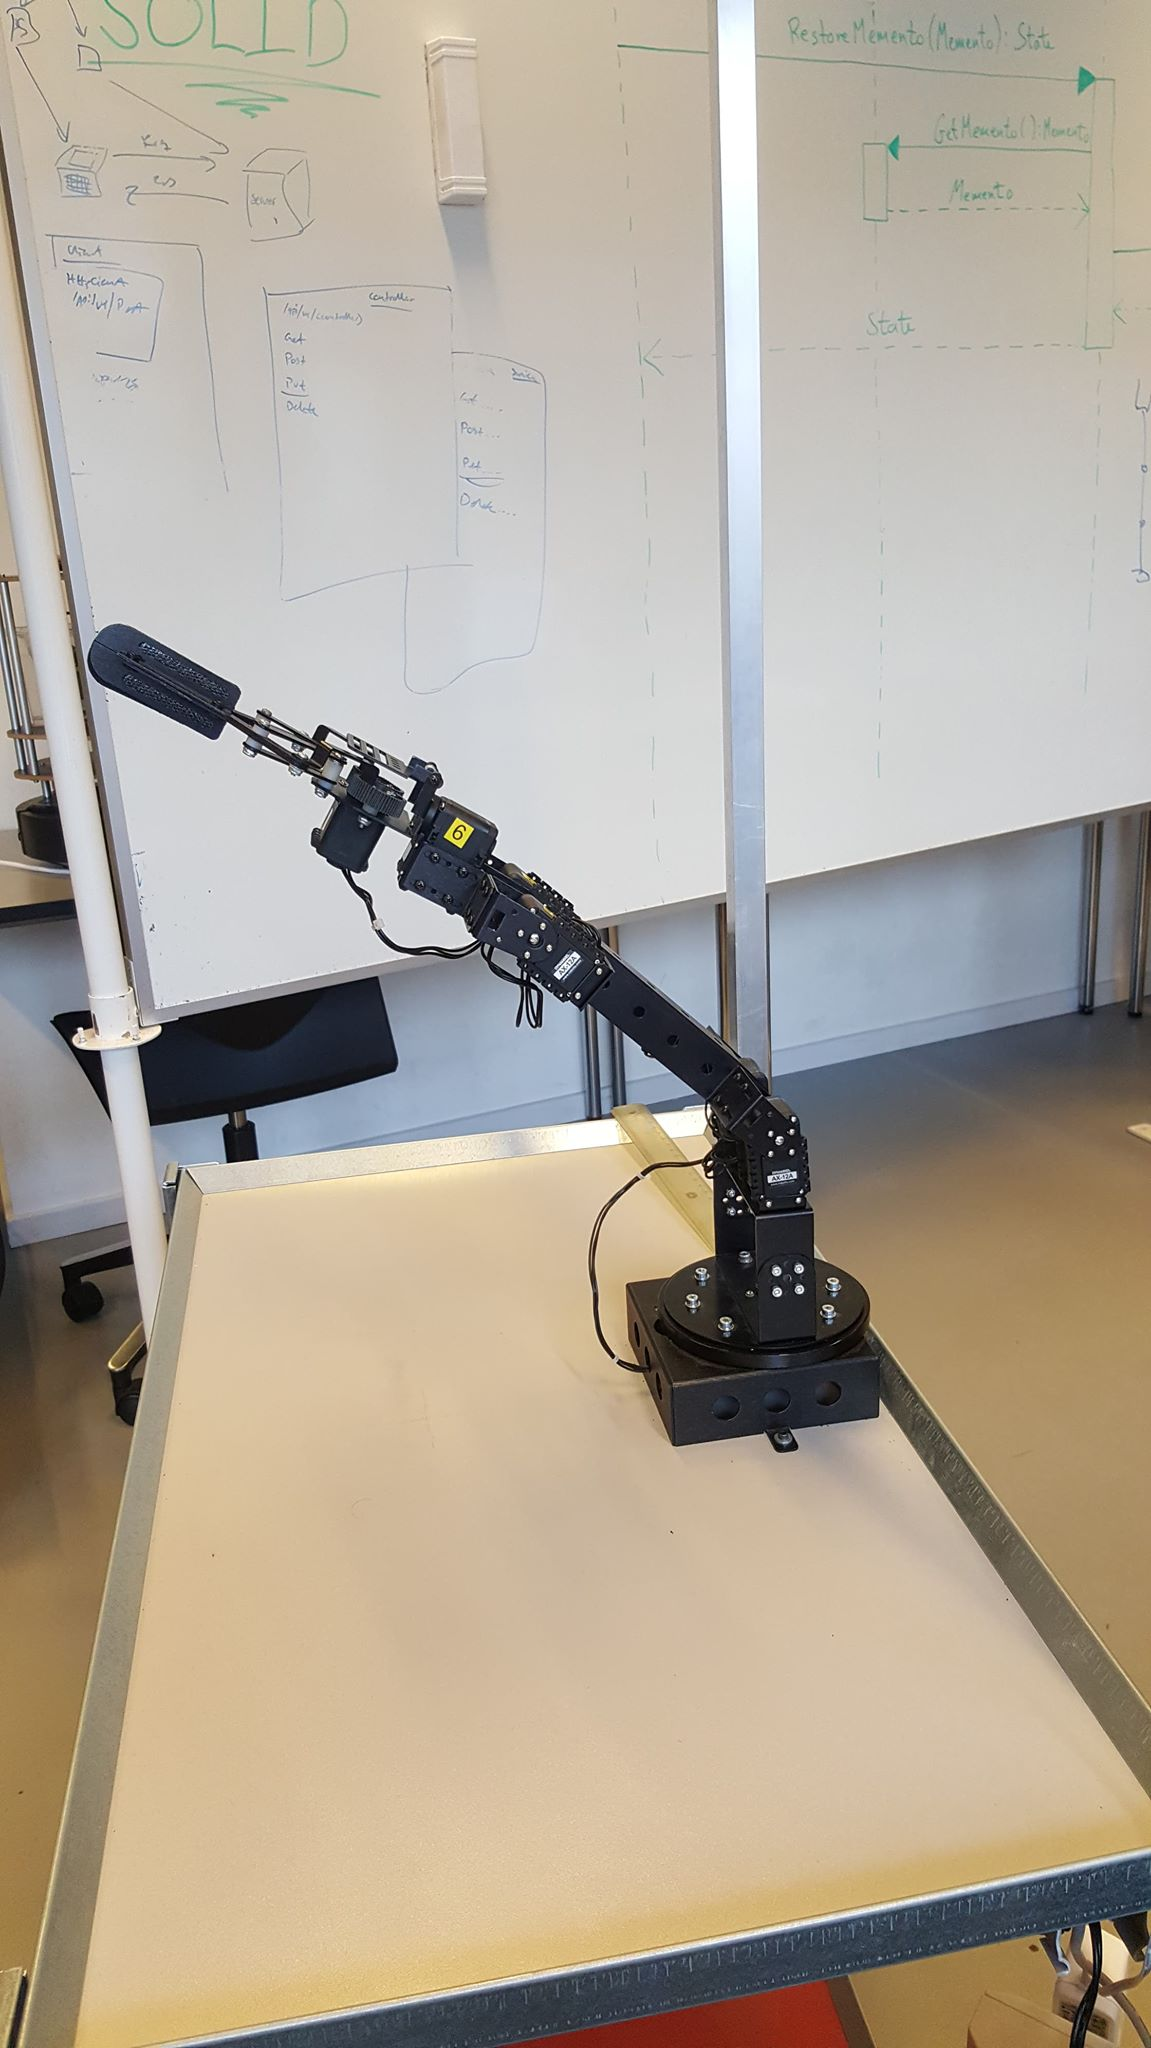
\includegraphics[width=0.4\textwidth,trim={0 20cm 0 18cm},clip]{figures/Matlab.jpg}
    \caption{Crustcrawler in a direction that was pretested in Matlab}
    \label{fig:matlab}
\end{figure}

The three figures below is used to test the robot stretched out in each of the three axes. The first height (d1) cannot be leaned forward, which means it will always point upwards along the z-axis. This means that the furthest the arm can reach in the x- and y-axis is the total length minus d1. The inverse kinematics coordinates of the robot, that are seen on the three figures, are respectively: \newline
[37, 0, 13] \newline
[0, 37, 13] \newline
[0, 0, 50]

\begin{figure}[H]
    \centering
    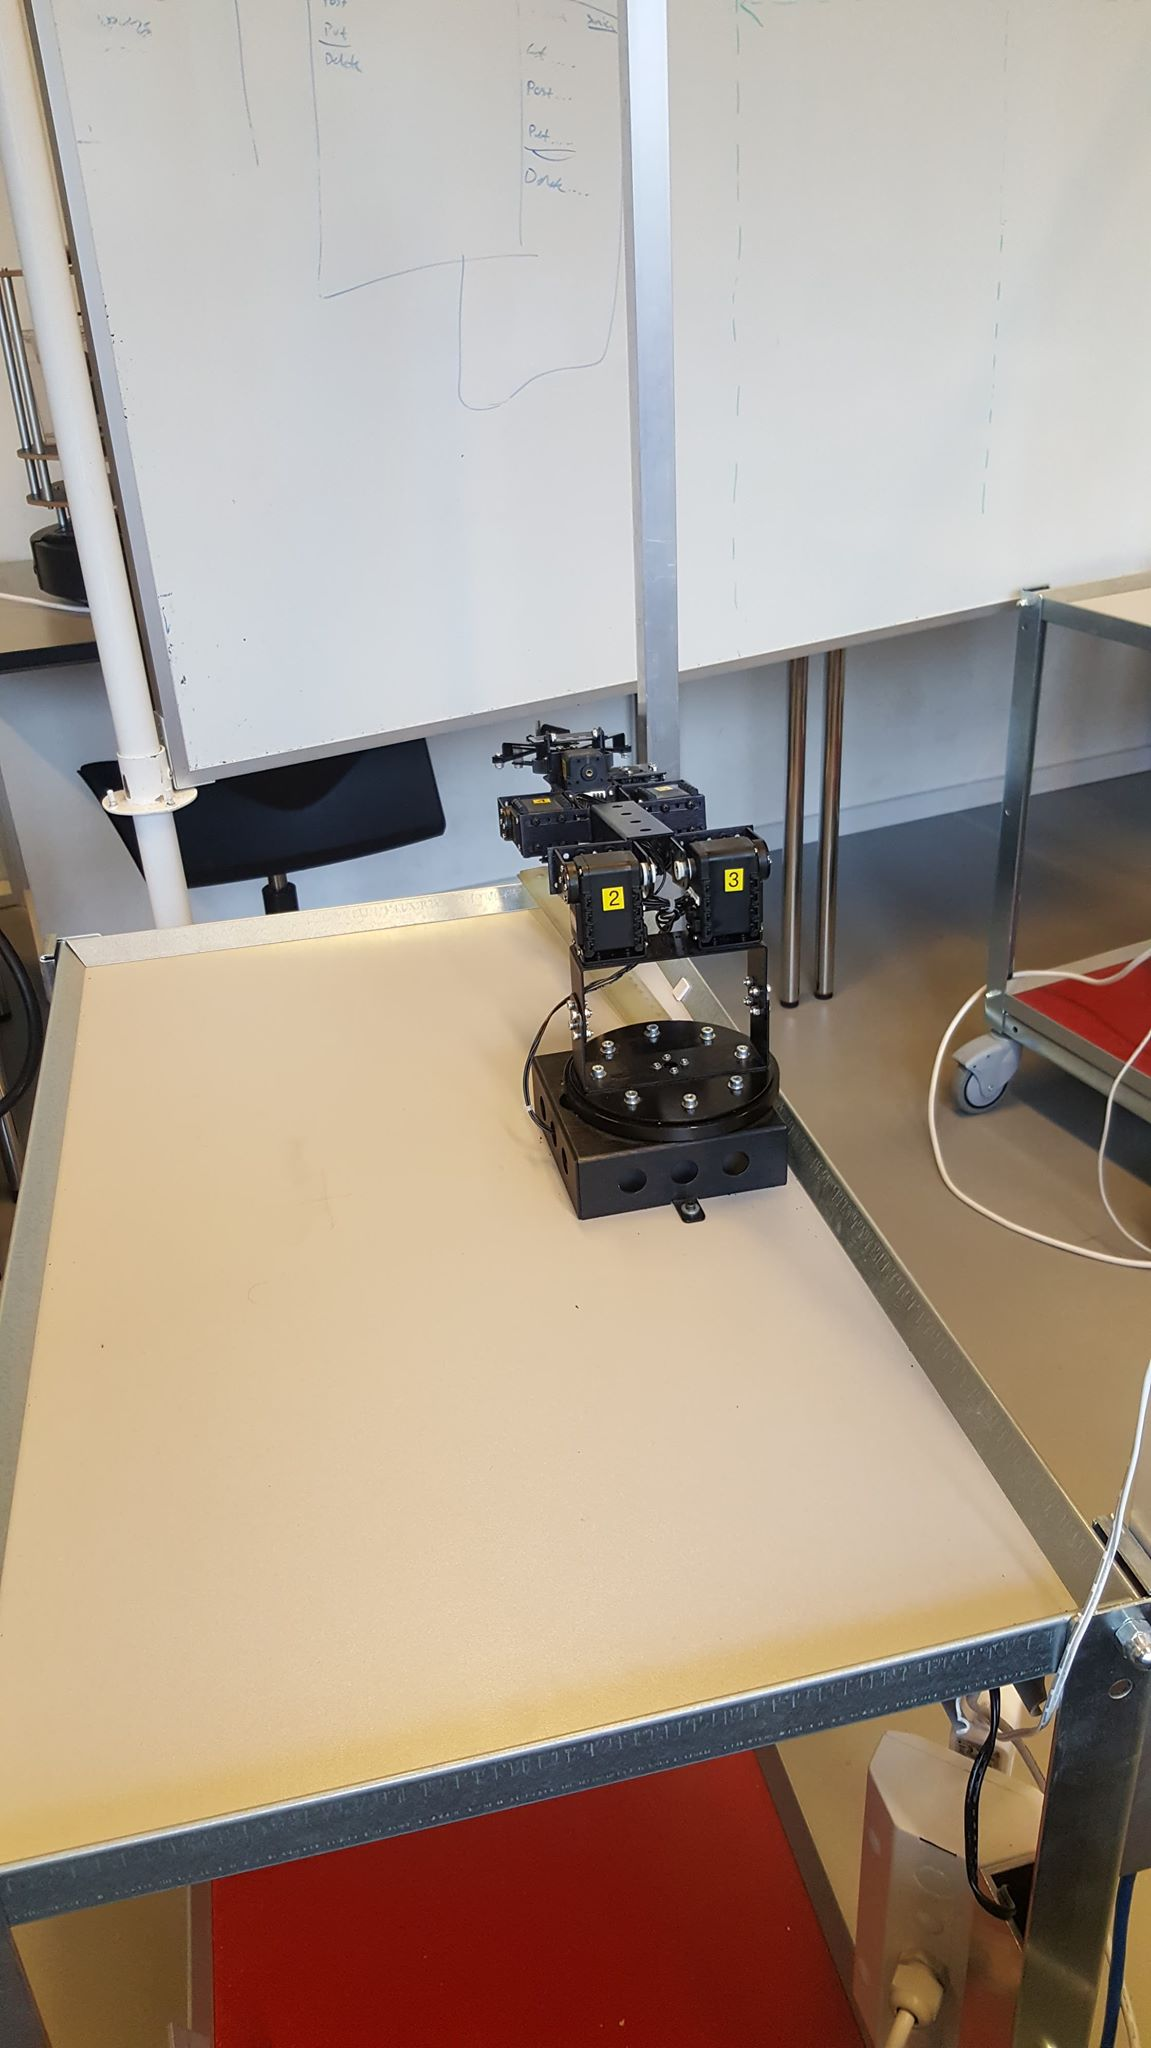
\includegraphics[width=0.4\textwidth,trim={0 25cm 0 18cm},clip]{figures/x.jpg}
    \caption{The Crustcrawler demonstrating it can point in the direction of the x-axis.}
    \label{fig:my_label}
\end{figure}

\begin{figure}[H]
    \centering
    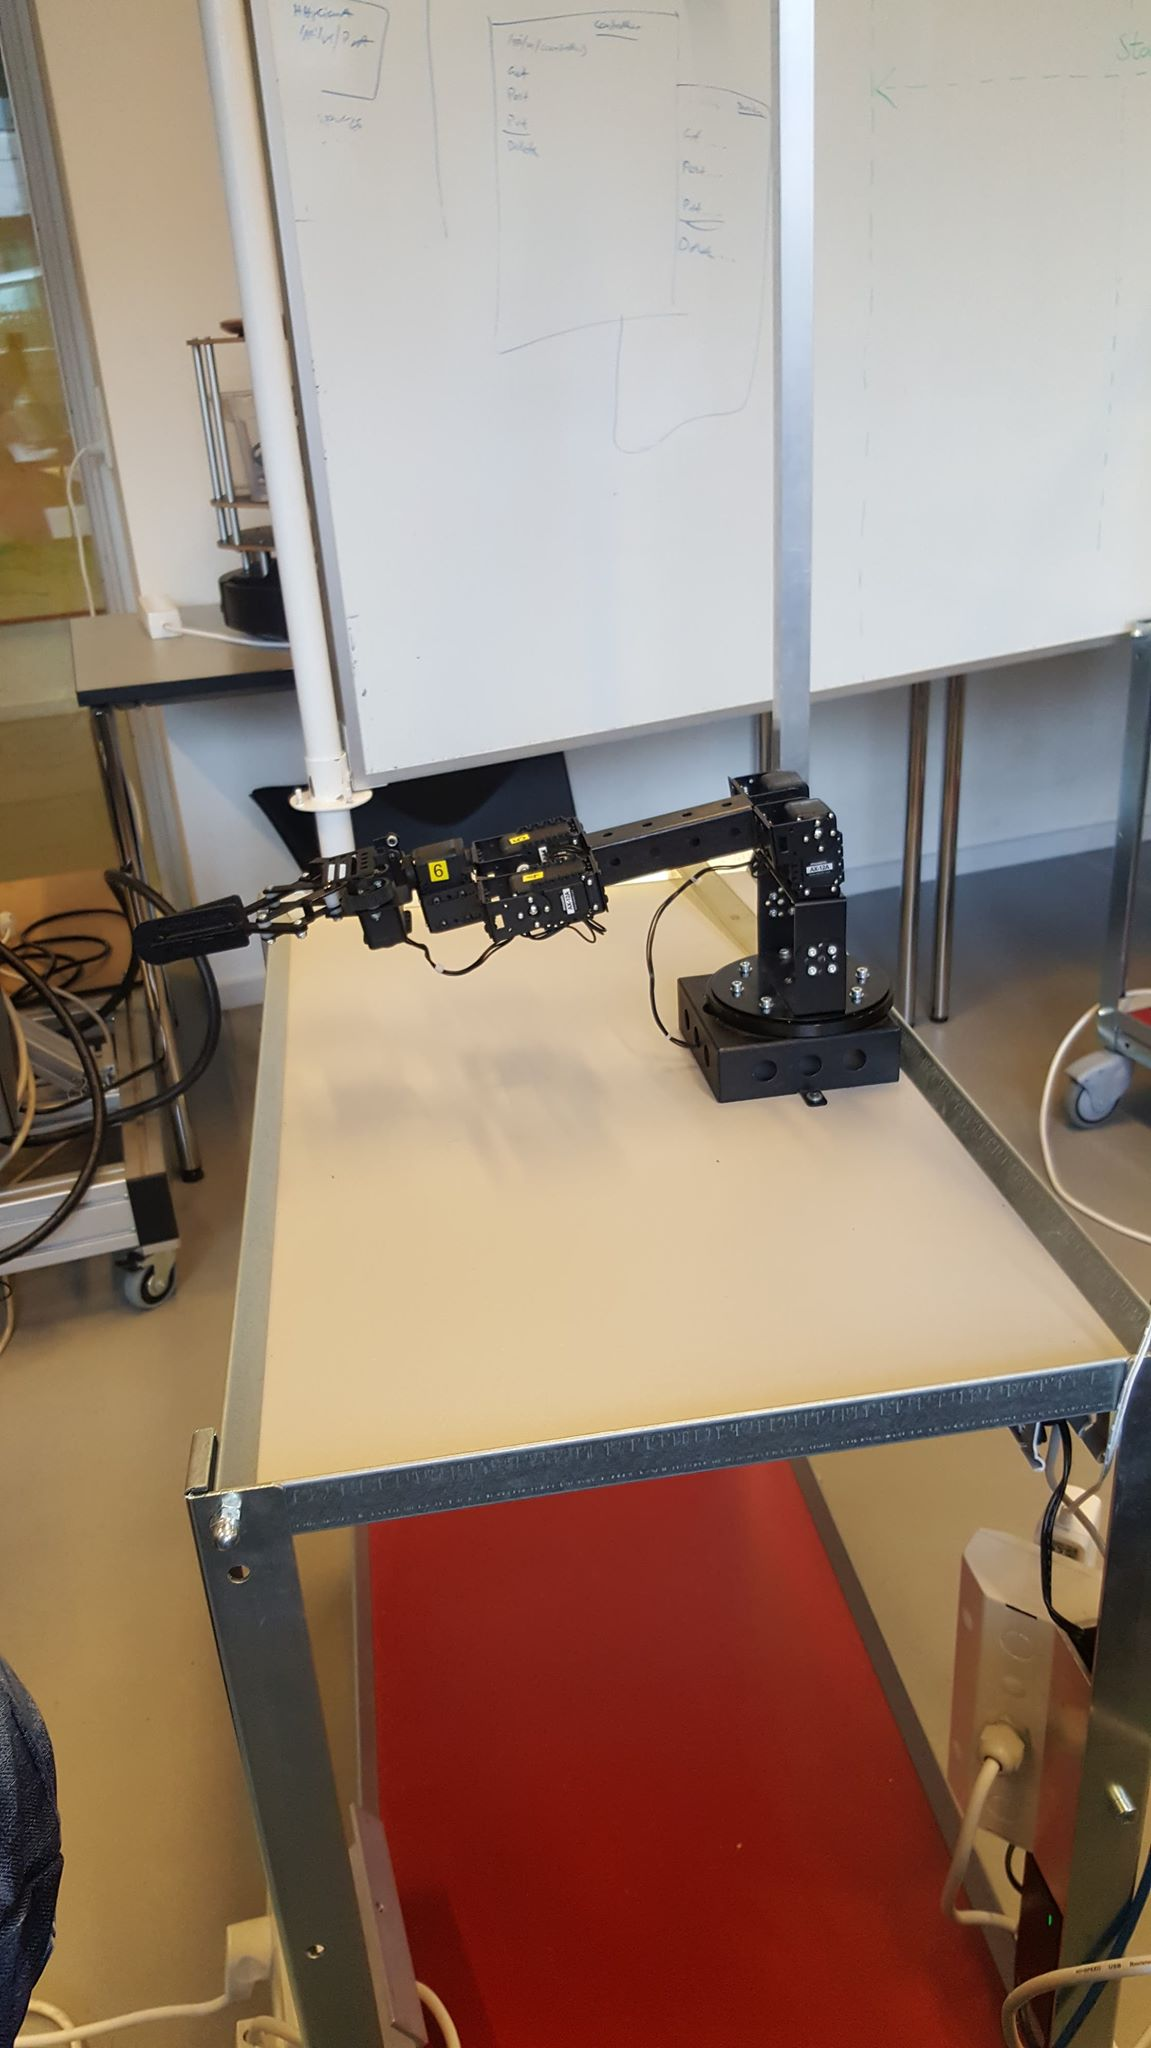
\includegraphics[width=0.4\textwidth,trim={0 25cm 0 18cm},clip]{figures/y.jpg}
    \caption{The Crustcrawler demonstrating it can point in the direction of the y-axis.}
    \label{fig:my_label}
\end{figure}

\begin{figure}[H]
    \centering
    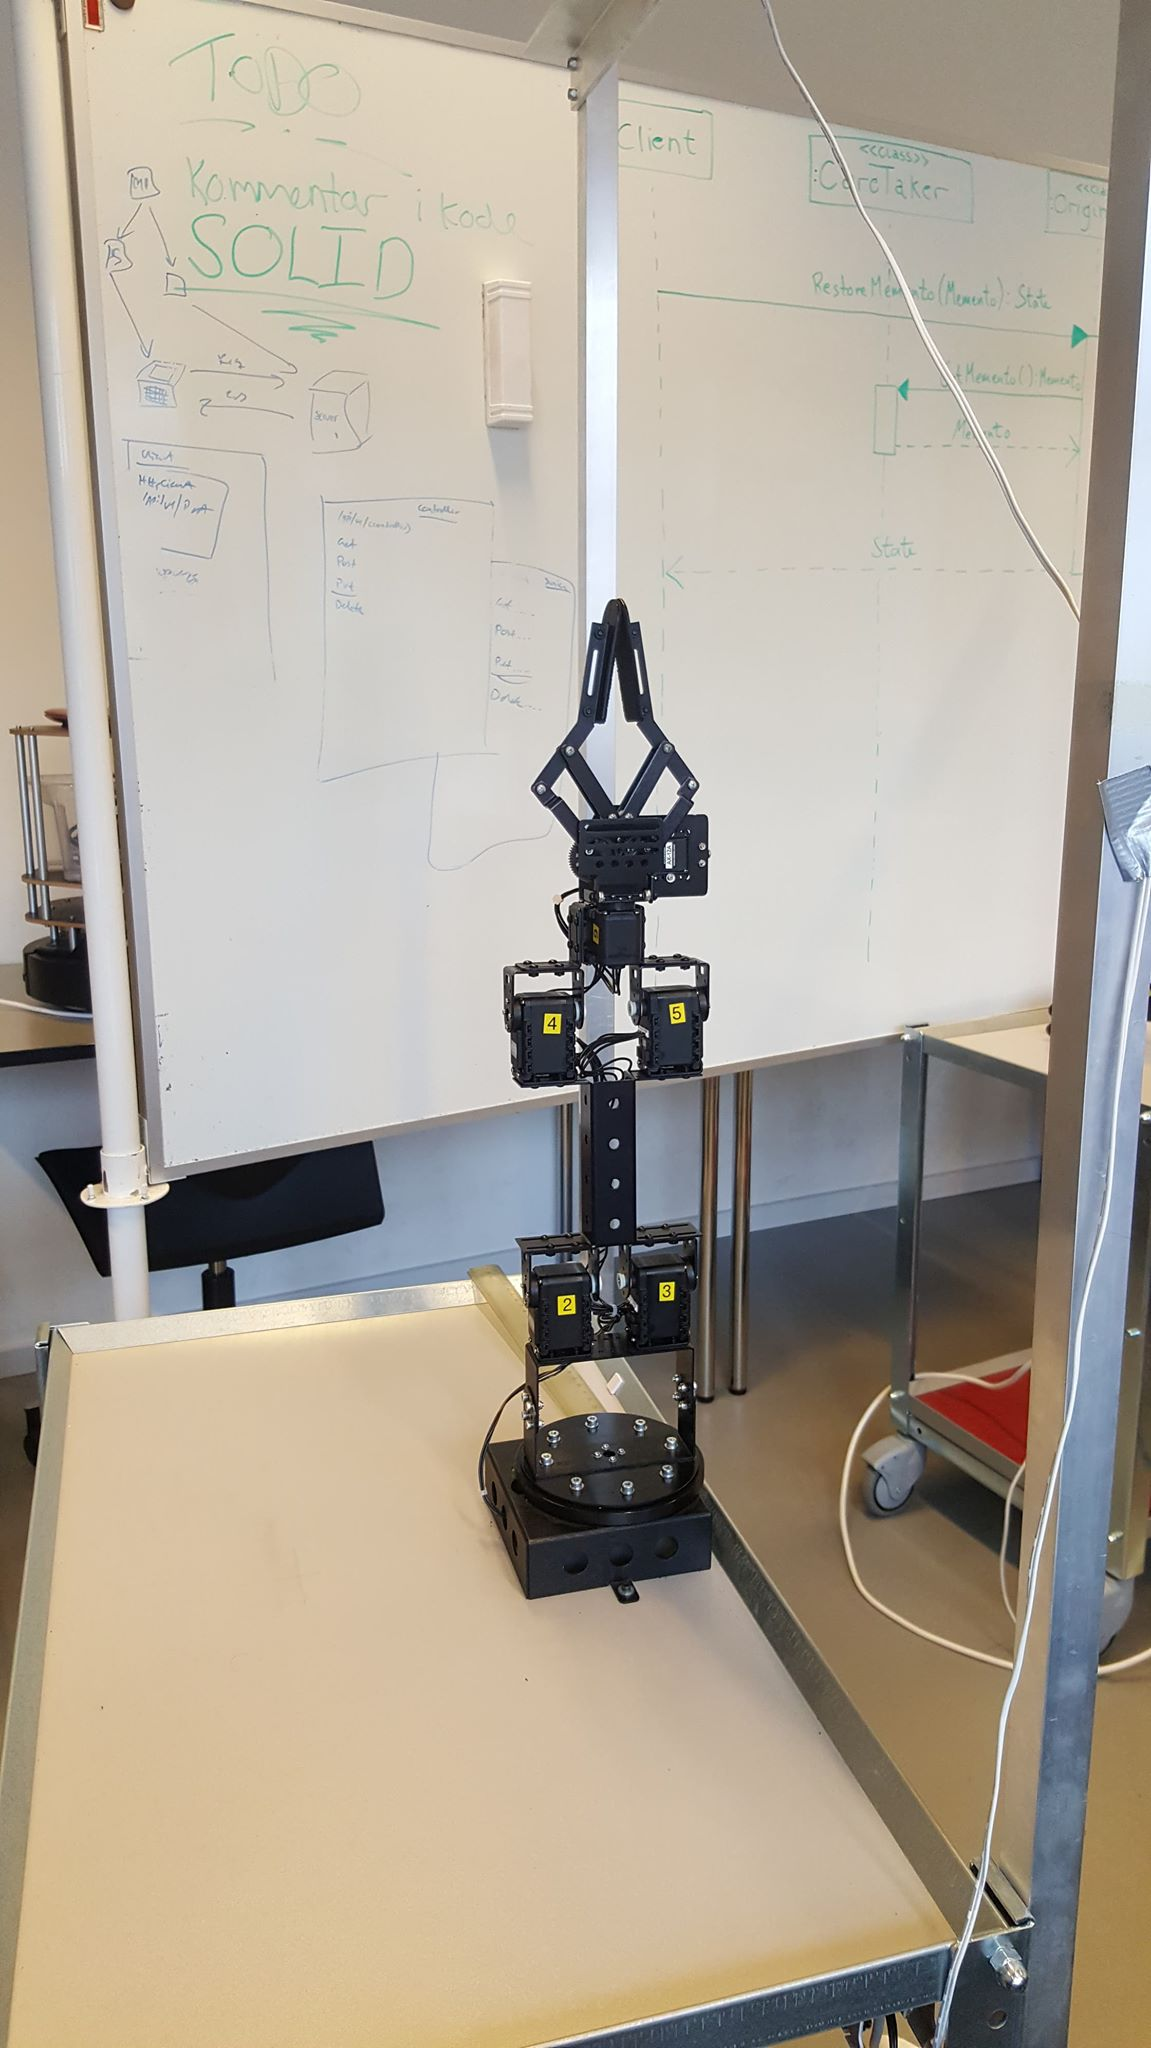
\includegraphics[width=0.4\textwidth,trim={0 15cm 0 18cm},clip]{figures/z.jpg}
    \caption{The Crustcrawler demonstrating it can point in the direction of the z-axis.}
    \label{fig:my_label}
\end{figure}

\subsection{Conclusion}

With this implementation of inverse kinematics we are now able to control the Crustcrawler to point to a specific location within its reachable 3d-space. This gives the robot a lot of controllability and makes it possible to handle objects with different locations.